\hypertarget{result-i-the-standard-model-as-a-selection-layer-a-demarcation}{%
\section{Result I --- the Standard Model as a selection layer (a demarcation)}\label{result-i-the-standard-model-as-a-selection-layer-a-demarcation}}

\hypertarget{the-problem-restated-structurally}{%
\subsection{The problem, restated structurally}\label{the-problem-restated-structurally}}

The Standard Model poses five ``why \textbf{this}?'' questions --- gauge group and representations, generation count and
textures, the electroweak scale, the vacuum, the UV completion. The calculus types all five as facets of \textbf{one
selection/measure layer} \(L^*\) sitting above the SM: a candidate-structure space \(W\) together with constraints and a
selection, of which the realized SM is a single point. The structural finding that frames everything else is that the
selection is \textbf{non-descending}: no function of the realized SM's own values determines the selection (computed
obstruction witnesses; a derived observable control \emph{does} descend, so the test discriminates).

This reframes the question. One does not \emph{derive} a selection from inside its own layer; one asks \textbf{which features of
the selected point are forced by structure, and which are irreducibly contingent} --- and proves the split. The honest
answer to ``why this whole SM?'' is a \emph{factorization}:

\[
\text{SM} \;=\; \underbrace{\text{[features closure forces or grounds]}}_{\text{few, listed below}}
\;\oplus\;
\underbrace{\text{[features provably invisible to closure]}}_{\text{observed-input, \emph{proved} so}} .
\]

This is the Galois genre of result: the point is the sharp, non-circular line, in both directions.

\hypertarget{unconditional-exclusion-sim-99.3-of-chiral-gauge-structures}{%
\subsection{\texorpdfstring{Unconditional exclusion: \(\sim 99.3\%\) of chiral gauge structures}{Unconditional exclusion: \textbackslash sim 99.3\textbackslash\% of chiral gauge structures}}\label{unconditional-exclusion-sim-99.3-of-chiral-gauge-structures}}

On a neutral carrier of \(11{,}990\) genuinely-chiral gauge structures (built token-blind: no SM labels appear in any
predicate; the realized SM-analog is report-only), the closure chain --- anomaly freedom~\citep{Bouchiat1972}, descent, corrected chirality,
mass-closure --- \textbf{excludes all but a small family}, leaving essentially the two-factor \(2|3\) class and a single-factor
\(SU(4)\) class. No condition is imposed beyond neutrality of the machinery; the exclusion is unconditional
(\textbf{COMPUTE}). Named competitors run through the same filter: \(SU(5)\) and flipped \(SU(5)\) fail at mass-closure;
Pati--Salam~\citep{PatiSalam1974}, left--right, and trinification are excluded by route-completeness within the declared component cap
(cap-conditional, stated as such); \(SO(10)\)/\(E_6\)~\citep{FritzschMinkowski1975} are outside the declared alphabet (not refuted).

\hypertarget{conditional-selection-of-mathfraksu2oplusmathfraksu3oplusmathfraku1}{%
\subsection{\texorpdfstring{Conditional selection of \(\mathfrak{su}(2)\oplus\mathfrak{su}(3)\oplus\mathfrak{u}(1)\)}{Conditional selection of \textbackslash mathfrak\{su\}(2)\textbackslash oplus\textbackslash mathfrak\{su\}(3)\textbackslash oplus\textbackslash mathfrak\{u\}(1)}}\label{conditional-selection-of-mathfraksu2oplusmathfraksu3oplusmathfraku1}}

One declared condition separates the survivors: \textbf{clean separation} --- the absence of confining-charged broken vectors.
In calculus terms it is the emptiness of a factorization defect: writing \(\pi_0\) for the confining readout and \(\pi_1\)
for the mass/breaking readout on the gauge bosons of a candidate structure,

\[
\text{clean separation} \iff \Delta_{\mathrm{fact}} = \varnothing ,
\]

and the witnesses of \(\Delta_{\mathrm{fact}}\neq\varnothing\) are exactly the \(X/Y\)-type colored coset bosons. Demanding
clean separation selects \(SU(2)\times SU(3)\times U(1)\) over the single-factor alternative (\textbf{SELECT}, on one named
condition). The single-factor side has since been upgraded to a constructed theorem: \emph{a single \(SU(N)\) with a stable
confining substrate has \(\Delta_{\mathrm{fact}}\neq\varnothing\) for all \(N\)} (symbolic three-step proof from the frozen
machinery; non-vacuous at \(N=4\)).

\hypertarget{the-xy-coset-spine-and-the-recovered-unification-ratios}{%
\subsection{\texorpdfstring{The \(X/Y\)-coset spine and the recovered unification ratios}{The X/Y-coset spine and the recovered unification ratios}}\label{the-xy-coset-spine-and-the-recovered-unification-ratios}}

The same defect object organizes a cluster of phenomena usually treated separately:

\begin{quote}
\textbf{One object, four roles.} The \(X/Y\) colored coset is simultaneously (i) the clean-separation violator, (ii) the
proton-decay mediator~\citep{Langacker1981} (its absence makes baryon number an F27 orbit-descent invariant: \(\mathcal O = 0\)), (iii) the
monopole source~\citep{Dirac1931,tHooft1974monopole} (its absence zeroes the F48 gluing obstruction), and (iv) the witness that a grand-unified parent is
a genuine refinement of the SM rather than a relabeling: \(\Delta_{\mathrm{fact}}(\mathrm{SM},\mathrm{GUT}) = 15\),
\(\Delta_{\mathrm{fact}}(\mathrm{GUT},\mathrm{SM}) = 0\).
\end{quote}

\begin{figure}[tbp]
  \centering
  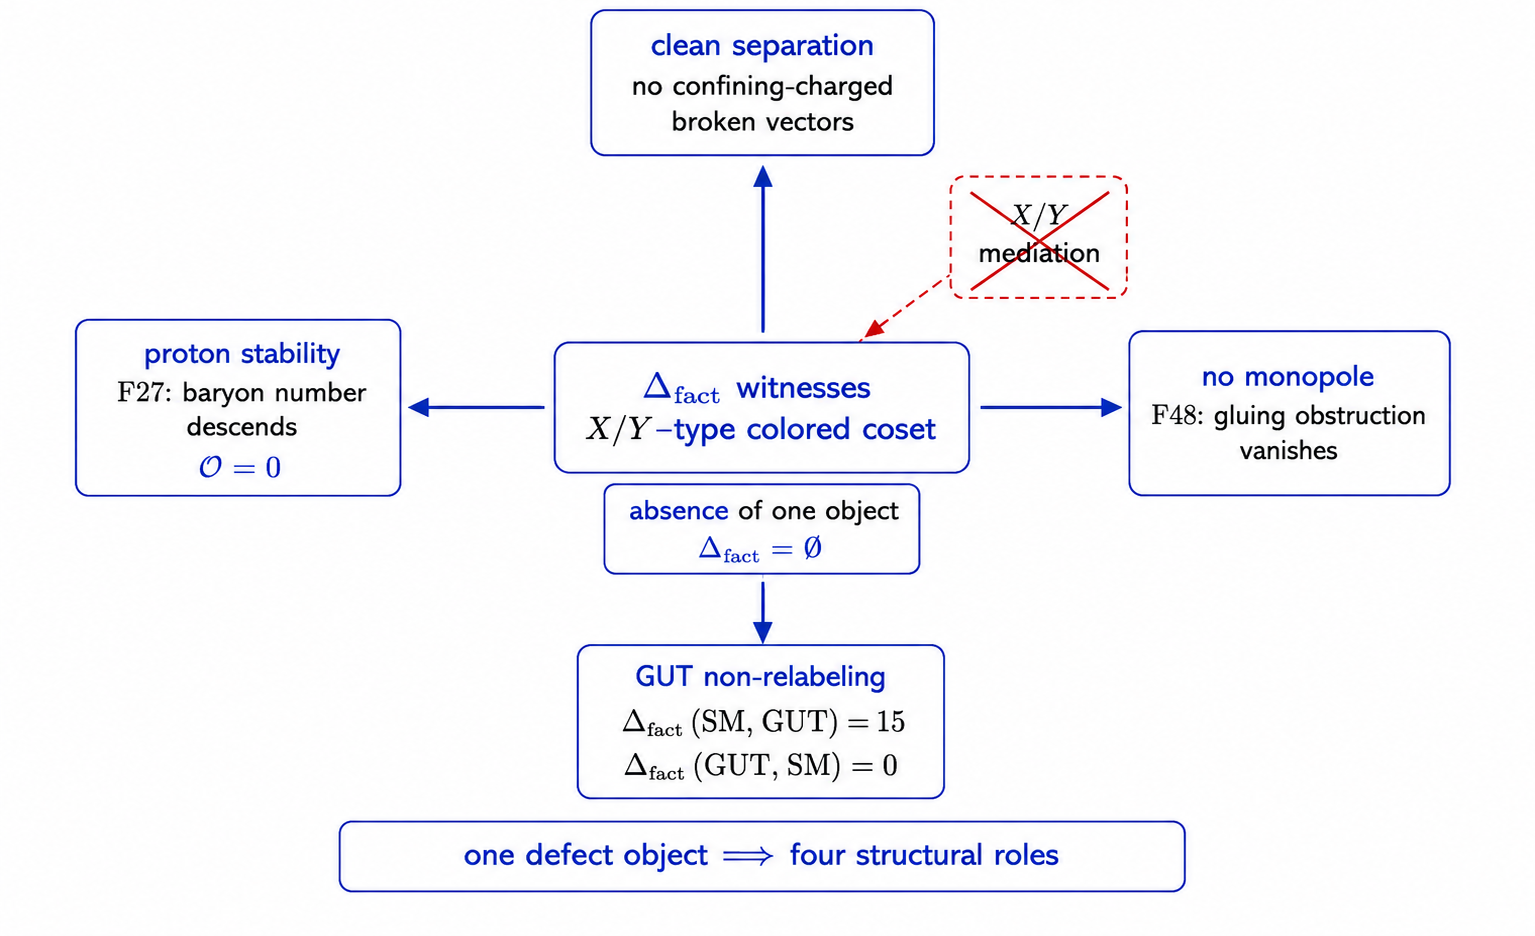
\includegraphics[width=0.7\linewidth]{figures/fig_f2_xy_coset_spine.png}
  \caption{\textbf{\(X/Y\)-coset spine.} \emph{One central node (\(\Delta_{\mathrm{fact}}\) witnesses) with four arrows --- clean-separation, proton stability (F27), no monopole (F48), GUT non-relabeling --- annotated ``absence of one object \(\Rightarrow\) all four at once.''}}
  \label{fig:f2}
\end{figure}

Constructing the F51 common-refinement parent over the SM's two routes lands the embedding numbers \textbf{as computations,
not inputs}. Over one SM generation,

\[
\sin^2\theta_W \;=\; \frac{\operatorname{Tr} T_3^2}{\operatorname{Tr} Q^2}
\;=\; \frac{2}{16/3} \;=\; \frac{3}{8},
\qquad
k_Y \;=\; \frac{5}{3} \ \ \text{(from } \operatorname{Tr} Y^2 = \tfrac{5}{6}\text{)} ,
\]

with the traces computed from the SM charge table (declared input) and the \emph{minimal-simple} parent class (declared
source). Non-circularity has a computed control: a product parent satisfying the same bare requirement yields \(3/23\),
so the value \(3/8\) genuinely depends on the declared source rather than being baked in (\textbf{GROUND}, conditional on that
source). Scope is strict: these are the \emph{embedding} ratios; the measured low-energy \(\sin^2\theta_W\) requires
renormalization-group running to a physical scale, which the toy does not contain --- and the flagship unification test
\textbf{fails} for minimal non-supersymmetric \(SU(5)\)~\citep{GeorgiGlashow1974}, consistent with experiment~\citep{SuperK2020}.

\hypertarget{grounding-the-condition-record-stability}{%
\subsection{Grounding the condition: record-stability}\label{grounding-the-condition-record-stability}}

Clean separation itself is not toy-derivable (the only internal grounding is circular --- caught and rejected). It is
\textbf{grounded one layer up} (\textbf{GROUND}): requiring a \emph{memory/record-stability} layer --- a stable confining substrate, the
capacity for at least two neutral records, and distinguishability --- \textbf{forces} clean separation. On the full carrier:

\[
\#\{\,\text{record-stable} \wedge \Delta_{\mathrm{fact}}\neq\varnothing\,\} \;=\; 0
\quad\text{out of } 11{,}990 .
\]

Anti-circularity is computed, not asserted: the substrate conjunct alone admits \(60\) decaying structures, the capacity
conjunct alone admits \(311\); only the conjunction lands in the clean class, and record-stability is \emph{not} extensionally
clean-separation (\(24\) record-stable structures versus \(316\) clean --- a strict directional implication). The
all-structures theorem upgrade (lemma L60\(\to\)L64) remains open and is tracked as such.

\hypertarget{the-blindness-theorems-what-is-proved-observed-input}{%
\subsection{\texorpdfstring{The blindness theorems: what is \emph{proved} observed-input}{The blindness theorems: what is proved observed-input}}\label{the-blindness-theorems-what-is-proved-observed-input}}

The demarcation's other half is proof-grade negatives (\textbf{PROVE-BLIND}):

\begin{itemize}
\tightlist
\item
  \textbf{Generation count.} For an anomaly-free content unit with an even per-unit \(SU(2)\)-doublet count (the SM unit
  qualifies), every gate of the frozen closure chain is invariant in \(N_{\mathrm{gen}}\): anomaly coefficients scale
  linearly (\(N\cdot u\)), the Witten parity gate~\citep{Witten1982} depends only on \((N\cdot d)\bmod 2\), and the remaining gates are
  nonempty-gated. Hence the chain passes identically for \textbf{all} \(N \ge 1\) (constructed theorem; an odd-doublet control
  \emph{is} \(N\)-sensitive, so the hypothesis is load-bearing). The calculus cannot see \(N_{\mathrm{gen}}=3\); the only handle
  is the recognition-source bound \((N-1)(N-2)/2 > 0 \iff N \ge 3\) from CP violation~\citep{KobayashiMaskawa1973} --- observed-input.
\item
  \textbf{Content.} Within the selected gauge structure, three definitionally distinct neutral shadows (integer charge
  quantization of the color-singlet spectrum; Yukawa-texture connectivity; mass-matrix rank) are all blind to the
  SM-vs-alternative content classes: the detailed matter content is a contingency-class residual (F26).
\item
  \textbf{Scales and values.} The electroweak scale is reframed (not solved) as an F47 small-selector region (\(\approx 3.96\%\)); no measured low-energy observable is derived anywhere in the track.
\end{itemize}

\hypertarget{result-sm-summary-table}{%
\subsection{Summary table}\label{result-sm-summary-table}}

\begin{longtable}[]{@{}lll@{}}
\toprule
\begin{minipage}[b]{0.28\columnwidth}\raggedright
question\strut
\end{minipage} & \begin{minipage}[b]{0.31\columnwidth}\raggedright
verdict (grade)\strut
\end{minipage} & \begin{minipage}[b]{0.34\columnwidth}\raggedright
basis\strut
\end{minipage}\tabularnewline
\midrule
\endhead
\begin{minipage}[t]{0.28\columnwidth}\raggedright
exclude \(\sim99.3\%\) of chiral gauge structures\strut
\end{minipage} & \begin{minipage}[t]{0.31\columnwidth}\raggedright
\textbf{COMPUTE}, unconditional\strut
\end{minipage} & \begin{minipage}[t]{0.34\columnwidth}\raggedright
closure chain on \(11{,}990\) structures\strut
\end{minipage}\tabularnewline
\begin{minipage}[t]{0.28\columnwidth}\raggedright
select \(\mathfrak{su}(2)\oplus\mathfrak{su}(3)\oplus\mathfrak{u}(1)\)\strut
\end{minipage} & \begin{minipage}[t]{0.31\columnwidth}\raggedright
\textbf{SELECT}, on clean separation\strut
\end{minipage} & \begin{minipage}[t]{0.34\columnwidth}\raggedright
\(\Delta_{\mathrm{fact}}=\varnothing\)\strut
\end{minipage}\tabularnewline
\begin{minipage}[t]{0.28\columnwidth}\raggedright
proton stability \(+\) no monopole \(+\) color separation\strut
\end{minipage} & \begin{minipage}[t]{0.31\columnwidth}\raggedright
\textbf{COMPUTE}\strut
\end{minipage} & \begin{minipage}[t]{0.34\columnwidth}\raggedright
one object: the \(X/Y\) coset, absent\strut
\end{minipage}\tabularnewline
\begin{minipage}[t]{0.28\columnwidth}\raggedright
\(\sin^2\theta_W = 3/8\), \(k_Y = 5/3\)\strut
\end{minipage} & \begin{minipage}[t]{0.31\columnwidth}\raggedright
\textbf{GROUND} (minimal-simple parent)\strut
\end{minipage} & \begin{minipage}[t]{0.34\columnwidth}\raggedright
trace ratios; product control \(3/23\)\strut
\end{minipage}\tabularnewline
\begin{minipage}[t]{0.28\columnwidth}\raggedright
clean separation itself\strut
\end{minipage} & \begin{minipage}[t]{0.31\columnwidth}\raggedright
\textbf{GROUND} (record-stability)\strut
\end{minipage} & \begin{minipage}[t]{0.34\columnwidth}\raggedright
\(0/11{,}990\) counterexamples; non-circular\strut
\end{minipage}\tabularnewline
\begin{minipage}[t]{0.28\columnwidth}\raggedright
single-factor exclusion, all \(N\)\strut
\end{minipage} & \begin{minipage}[t]{0.31\columnwidth}\raggedright
\textbf{COMPUTE} (constructed theorem)\strut
\end{minipage} & \begin{minipage}[t]{0.34\columnwidth}\raggedright
symbolic proof\strut
\end{minipage}\tabularnewline
\begin{minipage}[t]{0.28\columnwidth}\raggedright
\(N_{\mathrm{gen}}\), content, measured values\strut
\end{minipage} & \begin{minipage}[t]{0.31\columnwidth}\raggedright
\textbf{PROVE-BLIND} / observed-input\strut
\end{minipage} & \begin{minipage}[t]{0.34\columnwidth}\raggedright
all-\(N\) theorem; three blind shadows\strut
\end{minipage}\tabularnewline
\begin{minipage}[t]{0.28\columnwidth}\raggedright
measured \(\sin^2\theta_W\), couplings, masses, EW scale\strut
\end{minipage} & \begin{minipage}[t]{0.31\columnwidth}\raggedright
\textbf{not landed} (out of scope)\strut
\end{minipage} & \begin{minipage}[t]{0.34\columnwidth}\raggedright
need running/scale = experiment\strut
\end{minipage}\tabularnewline
\bottomrule
\end{longtable}

The Standard Model, on this evidence, is not one derivable object. It is a \emph{selection} with a thin forced skeleton ---
and the calculus proves both the skeleton and the thinness. Section 6.3 turns the spine of this analysis into a
falsifiable prediction.
